% Options for packages loaded elsewhere
\PassOptionsToPackage{unicode}{hyperref}
\PassOptionsToPackage{hyphens}{url}
%
\documentclass[
]{article}
\usepackage{amsmath,amssymb}
\usepackage{iftex}
\ifPDFTeX
  \usepackage[T1]{fontenc}
  \usepackage[utf8]{inputenc}
  \usepackage{textcomp} % provide euro and other symbols
\else % if luatex or xetex
  \usepackage{unicode-math} % this also loads fontspec
  \defaultfontfeatures{Scale=MatchLowercase}
  \defaultfontfeatures[\rmfamily]{Ligatures=TeX,Scale=1}
\fi
\usepackage{lmodern}
\ifPDFTeX\else
  % xetex/luatex font selection
\fi
% Use upquote if available, for straight quotes in verbatim environments
\IfFileExists{upquote.sty}{\usepackage{upquote}}{}
\IfFileExists{microtype.sty}{% use microtype if available
  \usepackage[]{microtype}
  \UseMicrotypeSet[protrusion]{basicmath} % disable protrusion for tt fonts
}{}
\makeatletter
\@ifundefined{KOMAClassName}{% if non-KOMA class
  \IfFileExists{parskip.sty}{%
    \usepackage{parskip}
  }{% else
    \setlength{\parindent}{0pt}
    \setlength{\parskip}{6pt plus 2pt minus 1pt}}
}{% if KOMA class
  \KOMAoptions{parskip=half}}
\makeatother
\usepackage{xcolor}
\usepackage[margin=1in]{geometry}
\usepackage{longtable,booktabs,array}
\usepackage{calc} % for calculating minipage widths
% Correct order of tables after \paragraph or \subparagraph
\usepackage{etoolbox}
\makeatletter
\patchcmd\longtable{\par}{\if@noskipsec\mbox{}\fi\par}{}{}
\makeatother
% Allow footnotes in longtable head/foot
\IfFileExists{footnotehyper.sty}{\usepackage{footnotehyper}}{\usepackage{footnote}}
\makesavenoteenv{longtable}
\usepackage{graphicx}
\makeatletter
\def\maxwidth{\ifdim\Gin@nat@width>\linewidth\linewidth\else\Gin@nat@width\fi}
\def\maxheight{\ifdim\Gin@nat@height>\textheight\textheight\else\Gin@nat@height\fi}
\makeatother
% Scale images if necessary, so that they will not overflow the page
% margins by default, and it is still possible to overwrite the defaults
% using explicit options in \includegraphics[width, height, ...]{}
\setkeys{Gin}{width=\maxwidth,height=\maxheight,keepaspectratio}
% Set default figure placement to htbp
\makeatletter
\def\fps@figure{htbp}
\makeatother
\setlength{\emergencystretch}{3em} % prevent overfull lines
\providecommand{\tightlist}{%
  \setlength{\itemsep}{0pt}\setlength{\parskip}{0pt}}
\setcounter{secnumdepth}{-\maxdimen} % remove section numbering
\ifLuaTeX
  \usepackage{selnolig}  % disable illegal ligatures
\fi
\usepackage{bookmark}
\IfFileExists{xurl.sty}{\usepackage{xurl}}{} % add URL line breaks if available
\urlstyle{same}
\hypersetup{
  pdftitle={Environmental variables for the 2024 SEAK Pink Salmon Preseason Forecast},
  pdfauthor={Sara Miller},
  hidelinks,
  pdfcreator={LaTeX via pandoc}}

\title{Environmental variables for the\\
2024 SEAK Pink Salmon Preseason Forecast}
\author{Sara Miller}
\date{October 2024}

\begin{document}
\maketitle

\section{Objective}\label{objective}

The overall objective is to test a variety of temperature variables,
using satellite sea surface temperature (SST) data or Southeast Alaska
Coastal Monitoring project (SECM) data, within the forecasting model
framework to forecast the 2024 pink salmon harvest in southeast Alaska
(SEAK). This write-up is a summary of available SST variables based on
satellite data (i.e., average of May (May), the average over the months
of May through July (MJJ), the average over the months of April through
June (AMJ), or the average over the months of April through July (AMJJ)
from 1997 through 2024) over four regions of SEAK; Icy Strait, Icy and
Chatham Straits, northern southeast Alaska (NSEAK), and SEAK. This
write-up also includes a summary of SECM survey data from various months
(i.e., the average over the months of May, June, and July (MJJ)) at 20 m
depths of the SECM transects (i.e., Icy Strait and Upper Chatham
transects stations ISA, ISB, ISC, ISD, UCA, UCB, UCC, UCD) from 1997
through 2024.

\section{Methods}\label{methods}

\subsection{Satellite-derived SST
data}\label{satellite-derived-sst-data}

Satellite-derived sea surface temperature (SST) data from April 1997
through July 2024 were pulled from the `SST and SST Anomaly, NOAA Global
Coral Bleaching Monitoring, 5km, V.3.1, Monthly, 1985-Present' time
series
(\url{https://coastwatch.pfeg.noaa.gov/erddap/griddap/NOAA_DHW_monthly.html};
full citation in references). This satellite-derived SST data set was
then matched to pre-determined coordinates from four spatial regions
that corresponded with sixteen variables of interest (four regions; four
temporal variables per region).

\subsubsection{Satellite-derived SST
variables}\label{satellite-derived-sst-variables}

\textbf{Icy\_Strait\_SST\_May}: The Icy Strait region encompasses waters
of Icy Strait from the east end of Lemesurier Island to a line from
Point Couverden south to Point Augusta. This variable is the average SST
in May (Table 1; Figure 1; Figure 5a).

\textbf{Icy\_Strait\_SST\_MJJ}: The Icy Strait region encompasses waters
of Icy Strait from the east end of Lemesurier Island to a line from
Point Couverden south to Point Augusta. This variable is the average SST
in May through July (Table 1; Figure 1; Figure 5b).

\textbf{Icy\_Strait\_SST\_AMJ}: The Icy Strait region encompasses waters
of Icy Strait from the east end of Lemesurier Island to a line from
Point Couverden south to Point Augusta. This variable is the average SST
in April through June (Table 1; Figure 1; Figure 5c).

\textbf{Icy\_Strait\_SST\_AMJJ}: The Icy Strait region encompasses
waters of Icy Strait from the east end of Lemesurier Island to a line
from Point Couverden south to Point Augusta. This variable is the
average SST in April through July (Table 1; Figure 1; Figure 5d).

\textbf{Chatham\_SST\_May}: The Chatham and Icy Straits region
encompasses waters of Chatham and Icy Straits east of Lemesurier Island
to Point Couverden, and south to the approximate latitude of 56.025
degrees north (roughly Cape Decision off Kuiu Island) (Figure 2 and
Figure 5a; Table 2). This variable is the average SST in May.

\textbf{Chatham\_SST\_MJJ}: The Chatham and Icy Straits region
encompasses waters of Chatham and Icy Straits east of Lemesurier Island
to Point Couverden, south to the approximate latitude of 56.025 degrees
north (roughly Cape Decision off Kuiu Island) (Figure 2 and Figure 5b;
Table 2). This variable is the average SST in May through July.

\textbf{Chatham\_SST\_AMJ}: The Chatham and Icy Straits region
encompasses waters of Chatham and Icy Straits east of Lemesurier Island
to Point Couverden, south to the approximate latitude of 56.025 degrees
north (roughly Cape Decision off Kuiu Island) (Figure 2 and Figure 5c;
Table 2). This variable is the average SST in April through June.

\textbf{Chatham\_SST\_AMJJ}: The Chatham and Icy Straits region
encompasses waters of Chatham and Icy Straits east of Lemesurier Island
to Point Couverden, south to the approximate latitude of 56.025 degrees
north (roughly Cape Decision off Kuiu Island) (Figure 2 and Figure 5d;
Table 2). This variable is the average SST in April through July.

\textbf{NSEAK\_SST\_May}: The NSEAK region encompasses northern
Southeast Alaska from 59.475 to 56.075 degrees north latitude
(approximately Districts 9 through 15, and District 13 inside area only;
northern Southeast Inside subregion for Southeast Alaska (NSEI); Figure
3 and Figure 5a; Table 3). This variable is the average SST in May.

\textbf{NSEAK\_SST\_MJJ}: The NSEAK region encompasses northern
Southeast Alaska from 59.475 to 56.075 degrees north latitude
(approximately Districts 9 through 15, and District 13 inside area only;
northern Southeast Inside subregion for Southeast Alaska (NSEI); Figure
3 and Figure 5b; Table 3). This variable is the average SST in May
through July.

\textbf{NSEAK\_SST\_AMJ}: The NSEAK region encompasses northern
Southeast Alaska from 59.475 to 56.075 degrees north latitude
(approximately Districts 9 through 15, and District 13 inside area only;
northern Southeast Inside subregion for Southeast Alaska (NSEI); Figure
3 and Figure 5c; Table 3). This variable is the average SST in April
through June.

\textbf{NSEAK\_SST\_AMJJ}: The NSEAK region encompasses northern
Southeast Alaska from 59.475 to 56.075 degrees north latitude
(approximately Districts 9 through 15, and District 13 inside area only;
northern Southeast Inside subregion for Southeast Alaska (NSEI); Figure
3 and Figure 5d; Table 3). This variable is the average SST in April
through July.

\textbf{SEAK\_SST\_May}: The SEAK region encompasses Southeast Alaska
from 59.475 to 54.725 degrees north latitude (Figure 4 and Figure 5a;
Table 4). This variable is the average SST in May.

\textbf{SEAK\_SST\_MJJ}: The SEAK region encompasses northern Southeast
Alaska from 59.475 to 54.725 degrees north latitude (Figure 4 and Figure
5b; Table 4). This variable is the average SST in May through July.

\textbf{SEAK\_SST\_AMJ}: The SEAK region encompasses Southeast Alaska
from 59.475 to 54.725 degrees north latitude (Figure 4 and Figure 5c;
Table 4). This variable is the average SST in April through June.

\textbf{SEAK\_SST\_AMJJ}: The SEAK region encompasses Southeast Alaska
from 59.475 to 54.725 degrees north latitude (Figure 4 and Figure 5d;
Table 4). This variable is the average SST in April through July.

\subsection{SECM survey temperature
data}\label{secm-survey-temperature-data}

SECM survey temperature data were summarized by year (1997 to 2024),
month (average over the months of May, June, and July) at 20m depths for
the Icy Strait and Upper Chatham transects combined.

\subsubsection{SECM survey temperature
variables}\label{secm-survey-temperature-variables}

\textbf{ISTI20\_MJJ}: Average temperature in the upper 20m during May
through July at 8 stations in Icy Strait (Icy Strait and Upper Chatham
transects; Figure 1; Figure 6; Table 5).

\section{Results}\label{results}

\subsection{Satellite-derived SST
data}\label{satellite-derived-sst-data-1}

Satellite sea surface temperature data were summarized by region and
year (i.e., average of May (May), the average over the months of May,
June, and July (MJJ), the average over the months of April through June
(AMJ), or the average over the months of April through July (AMJJ)) from
1997 to 2024 (Tables 1 through 4).

\pagebreak

\begin{longtable}[]{@{}ccccc@{}}
\caption{Satellite sea temperature data from the Icy Strait region from
1997 to 2024 for the month of May (May), May through July (MJJ), April
through June (AMJ), and April through July (AMJJ). There are 70
satellite stations (latitude/longitude combinations) in the Icy Strait
region.}\tabularnewline
\toprule\noalign{}
year & Icy\_Strait\_SST\_MJJ & Icy\_Strait\_SST\_May &
Icy\_Strait\_SST\_AMJJ & Icy\_Strait\_SST\_AMJ \\
\midrule\noalign{}
\endfirsthead
\toprule\noalign{}
year & Icy\_Strait\_SST\_MJJ & Icy\_Strait\_SST\_May &
Icy\_Strait\_SST\_AMJJ & Icy\_Strait\_SST\_AMJ \\
\midrule\noalign{}
\endhead
\bottomrule\noalign{}
\endlastfoot
1997 & 10.30 & 7.01 & 8.83 & 7.30 \\
1998 & 9.97 & 7.34 & 8.85 & 7.56 \\
1999 & 9.08 & 6.17 & 8.02 & 6.78 \\
2000 & 9.94 & 7.02 & 8.67 & 7.35 \\
2001 & 9.57 & 6.48 & 8.40 & 7.08 \\
2002 & 9.34 & 6.26 & 8.02 & 6.60 \\
2003 & 10.08 & 7.29 & 8.88 & 7.53 \\
2004 & 10.68 & 7.53 & 9.25 & 7.69 \\
2005 & 11.16 & 8.40 & 9.64 & 8.26 \\
2006 & 10.19 & 6.84 & 8.86 & 7.49 \\
2007 & 9.49 & 6.55 & 8.16 & 6.87 \\
2008 & 8.85 & 6.43 & 7.72 & 6.68 \\
2009 & 9.94 & 7.19 & 8.47 & 7.22 \\
2010 & 9.87 & 7.71 & 8.68 & 7.81 \\
2011 & 9.84 & 6.81 & 8.47 & 7.18 \\
2012 & 9.23 & 6.92 & 8.10 & 7.07 \\
2013 & 9.88 & 6.37 & 8.45 & 6.97 \\
2014 & 10.23 & 7.90 & 8.81 & 7.62 \\
2015 & 10.73 & 8.34 & 9.43 & 8.29 \\
2016 & 11.65 & 8.81 & 10.37 & 9.14 \\
2017 & 9.82 & 7.22 & 8.66 & 7.51 \\
2018 & 9.99 & 6.92 & 8.74 & 7.43 \\
2019 & 10.74 & 7.79 & 9.51 & 8.10 \\
2020 & 10.40 & 7.83 & 9.05 & 7.86 \\
2021 & 10.26 & 6.91 & 8.91 & 7.47 \\
2022 & 10.34 & 7.13 & 8.88 & 7.40 \\
2023 & 9.72 & 7.13 & 8.43 & 7.10 \\
\end{longtable}

\pagebreak

\begin{longtable}[]{@{}ccccc@{}}
\caption{Satellite sea temperature data from the Chatham and Icy Straits
region from 1997 to 2024 for the month of May (May), May through July
(MJJ), April through June (AMJ), and April through July (AMJJ). There
are 313 satellite stations (latitude/longitude combinations) in the
Chatham and Icy Straits region.}\tabularnewline
\toprule\noalign{}
year & Chatham\_SST\_MJJ & Chatham\_SST\_May & Chatham\_SST\_AMJJ &
Chatham\_SST\_AMJ \\
\midrule\noalign{}
\endfirsthead
\toprule\noalign{}
year & Chatham\_SST\_MJJ & Chatham\_SST\_May & Chatham\_SST\_AMJJ &
Chatham\_SST\_AMJ \\
\midrule\noalign{}
\endhead
\bottomrule\noalign{}
\endlastfoot
1997 & 10.08 & 7.48 & 8.83 & 7.59 \\
1998 & 9.85 & 7.83 & 8.91 & 7.88 \\
1999 & 8.90 & 6.84 & 8.05 & 7.12 \\
2000 & 9.70 & 7.34 & 8.62 & 7.52 \\
2001 & 9.15 & 6.74 & 8.18 & 7.12 \\
2002 & 8.97 & 6.39 & 7.85 & 6.64 \\
2003 & 9.92 & 7.71 & 8.90 & 7.85 \\
2004 & 10.43 & 7.94 & 9.22 & 7.96 \\
2005 & 10.67 & 8.51 & 9.48 & 8.44 \\
2006 & 9.78 & 7.16 & 8.68 & 7.58 \\
2007 & 9.52 & 7.04 & 8.41 & 7.27 \\
2008 & 8.65 & 6.77 & 7.69 & 6.83 \\
2009 & 9.75 & 7.30 & 8.46 & 7.35 \\
2010 & 9.65 & 7.97 & 8.66 & 7.93 \\
2011 & 9.59 & 7.31 & 8.49 & 7.55 \\
2012 & 9.17 & 7.07 & 8.18 & 7.22 \\
2013 & 9.66 & 6.74 & 8.44 & 7.21 \\
2014 & 9.98 & 8.17 & 8.76 & 7.77 \\
2015 & 10.62 & 8.87 & 9.55 & 8.73 \\
2016 & 11.04 & 8.92 & 10.03 & 9.07 \\
2017 & 9.65 & 7.65 & 8.70 & 7.76 \\
2018 & 9.87 & 7.40 & 8.75 & 7.61 \\
2019 & 10.47 & 8.24 & 9.46 & 8.35 \\
2020 & 9.99 & 8.09 & 8.84 & 7.86 \\
2021 & 10.06 & 7.25 & 8.90 & 7.63 \\
2022 & 10.17 & 7.52 & 8.92 & 7.64 \\
2023 & 9.80 & 7.53 & 8.61 & 7.40 \\
\end{longtable}

\pagebreak

\begin{longtable}[]{@{}ccccc@{}}
\caption{Satellite sea temperature from the northern Southeast Alaska
(NSEAK) region from 1997 to 2024 for the month of May (May), May through
July (MJJ), April through June (AMJ), and April through July (AMJJ).
There are 1,344 satellite stations (latitude/longitude combinations) in
the NSEAK region.}\tabularnewline
\toprule\noalign{}
year & NSEAK\_SST\_MJJ & NSEAK\_SST\_May & NSEAK\_SST\_AMJJ &
NSEAK\_SST\_AMJ \\
\midrule\noalign{}
\endfirsthead
\toprule\noalign{}
year & NSEAK\_SST\_MJJ & NSEAK\_SST\_May & NSEAK\_SST\_AMJJ &
NSEAK\_SST\_AMJ \\
\midrule\noalign{}
\endhead
\bottomrule\noalign{}
\endlastfoot
1997 & 10.02 & 7.35 & 8.71 & 7.40 \\
1998 & 9.89 & 7.65 & 8.85 & 7.71 \\
1999 & 8.93 & 6.70 & 7.98 & 6.95 \\
2000 & 9.70 & 7.23 & 8.57 & 7.39 \\
2001 & 9.22 & 6.66 & 8.17 & 7.01 \\
2002 & 9.05 & 6.39 & 7.88 & 6.61 \\
2003 & 9.86 & 7.57 & 8.76 & 7.60 \\
2004 & 10.38 & 7.89 & 9.09 & 7.79 \\
2005 & 10.63 & 8.42 & 9.35 & 8.26 \\
2006 & 9.72 & 6.98 & 8.55 & 7.36 \\
2007 & 9.44 & 6.90 & 8.24 & 7.03 \\
2008 & 8.65 & 6.64 & 7.63 & 6.74 \\
2009 & 9.77 & 7.32 & 8.40 & 7.24 \\
2010 & 9.62 & 7.76 & 8.54 & 7.72 \\
2011 & 9.67 & 7.25 & 8.44 & 7.44 \\
2012 & 9.14 & 6.95 & 8.09 & 7.10 \\
2013 & 9.67 & 6.59 & 8.36 & 7.04 \\
2014 & 10.03 & 8.15 & 8.70 & 7.64 \\
2015 & 10.81 & 8.92 & 9.56 & 8.65 \\
2016 & 11.18 & 8.92 & 10.05 & 9.00 \\
2017 & 9.82 & 7.75 & 8.77 & 7.78 \\
2018 & 10.11 & 7.53 & 8.86 & 7.63 \\
2019 & 10.87 & 8.42 & 9.65 & 8.44 \\
2020 & 10.23 & 8.26 & 8.98 & 7.94 \\
2021 & 10.23 & 7.29 & 8.96 & 7.65 \\
2022 & 10.52 & 7.62 & 9.11 & 7.74 \\
2023 & 9.98 & 7.53 & 8.69 & 7.41 \\
\end{longtable}

\pagebreak

\begin{longtable}[]{@{}ccccc@{}}
\caption{Satellite sea temperature from the Southeast Alaska (SEAK)
region from 1997 to 2024 for the month of May (May), May through July
(MJJ), April through June (AMJ), and April through July (AMJJ). There
are 2,663 satellite stations (latitude/longitude combinations) in the
SEAK region.}\tabularnewline
\toprule\noalign{}
year & SEAK\_SST\_MJJ & SEAK\_SST\_May & SEAK\_SST\_AMJJ &
SEAK\_SST\_AMJ \\
\midrule\noalign{}
\endfirsthead
\toprule\noalign{}
year & SEAK\_SST\_MJJ & SEAK\_SST\_May & SEAK\_SST\_AMJJ &
SEAK\_SST\_AMJ \\
\midrule\noalign{}
\endhead
\bottomrule\noalign{}
\endlastfoot
1997 & 10.47 & 8.00 & 9.20 & 7.99 \\
1998 & 10.36 & 8.37 & 9.38 & 8.37 \\
1999 & 9.30 & 7.23 & 8.40 & 7.43 \\
2000 & 10.02 & 7.71 & 8.95 & 7.86 \\
2001 & 9.51 & 7.10 & 8.52 & 7.45 \\
2002 & 9.44 & 6.92 & 8.33 & 7.14 \\
2003 & 10.32 & 8.17 & 9.25 & 8.16 \\
2004 & 10.98 & 8.58 & 9.74 & 8.51 \\
2005 & 11.06 & 8.92 & 9.83 & 8.82 \\
2006 & 10.19 & 7.63 & 9.07 & 7.96 \\
2007 & 9.99 & 7.51 & 8.82 & 7.64 \\
2008 & 9.18 & 7.22 & 8.17 & 7.28 \\
2009 & 10.20 & 7.76 & 8.85 & 7.73 \\
2010 & 10.09 & 8.28 & 9.05 & 8.23 \\
2011 & 10.05 & 7.74 & 8.88 & 7.92 \\
2012 & 9.68 & 7.47 & 8.63 & 7.61 \\
2013 & 10.39 & 7.51 & 9.10 & 7.85 \\
2014 & 10.57 & 8.62 & 9.26 & 8.17 \\
2015 & 11.43 & 9.64 & 10.21 & 9.32 \\
2016 & 11.67 & 9.61 & 10.59 & 9.59 \\
2017 & 10.31 & 8.25 & 9.28 & 8.29 \\
2018 & 10.79 & 8.28 & 9.54 & 8.30 \\
2019 & 11.46 & 9.01 & 10.25 & 9.05 \\
2020 & 10.70 & 8.90 & 9.52 & 8.53 \\
2021 & 10.82 & 7.97 & 9.58 & 8.31 \\
2022 & 11.04 & 8.22 & 9.68 & 8.38 \\
2023 & 10.68 & 8.21 & 9.35 & 8.04 \\
\end{longtable}

\pagebreak

\subsection{SECM survey temperature
data}\label{secm-survey-temperature-data-1}

SECM survey temperature data were summarized by year (1997 to 2024),
month (average over the months of May, June, and July) at 20m depths;
Table 5).

Table: The SECM survey temperature data were summarized by year (1997 to
2024), month (the months of May, June, and July; MJJ) at 20m depths for
the Icy Strait and Upper Chatham transects (stations ISA, ISB, ISC, ISD,
UCA, UCB, UCC, UCD).

\begin{figure}
\centering
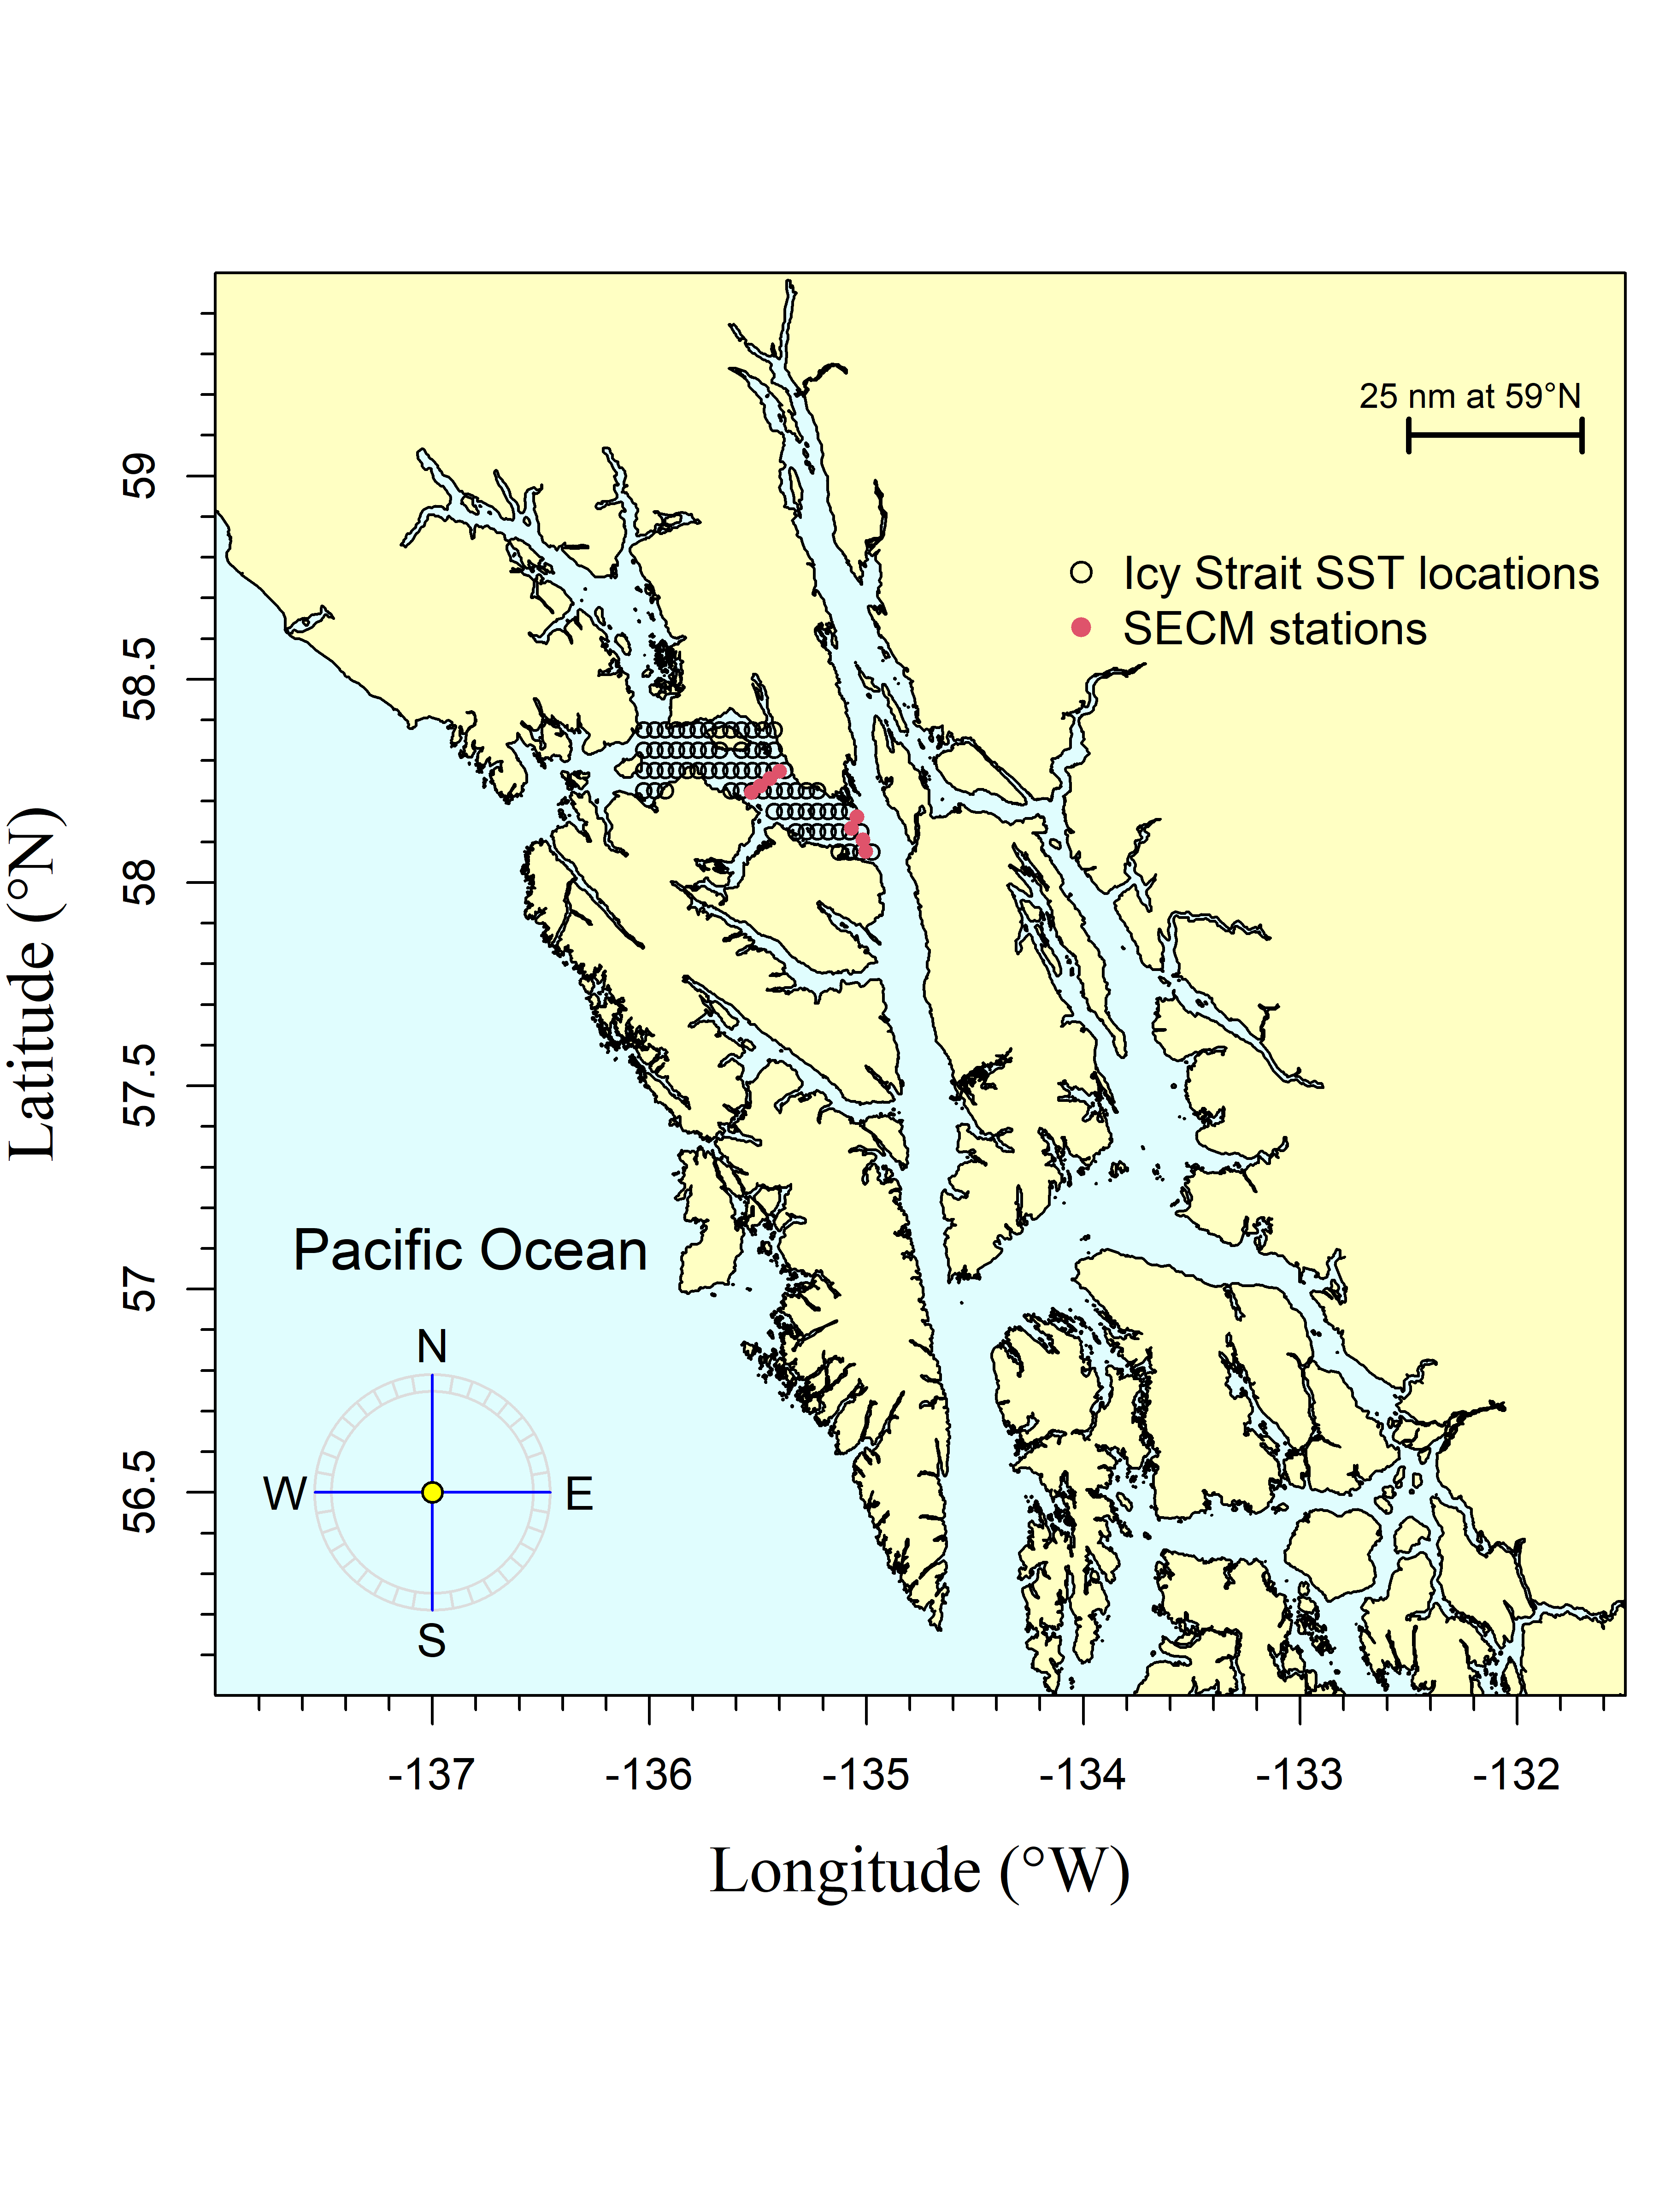
\includegraphics{../../2024_forecast/results/temperature_data/Icy_Strait.png}
\caption{The Icy Strait region encompasses waters of Icy Strait from the
east end of Lemesurier Island to a line from Point Couverden south to
Point Augusta. The Southeast Coastal Monitoring (SECM) project transects
(Upper Chatham Strait and Icy Strait) are shown as red points for
comparison to the satellite stations (i.e., data points; black
circles).}
\end{figure}

\begin{figure}
\centering
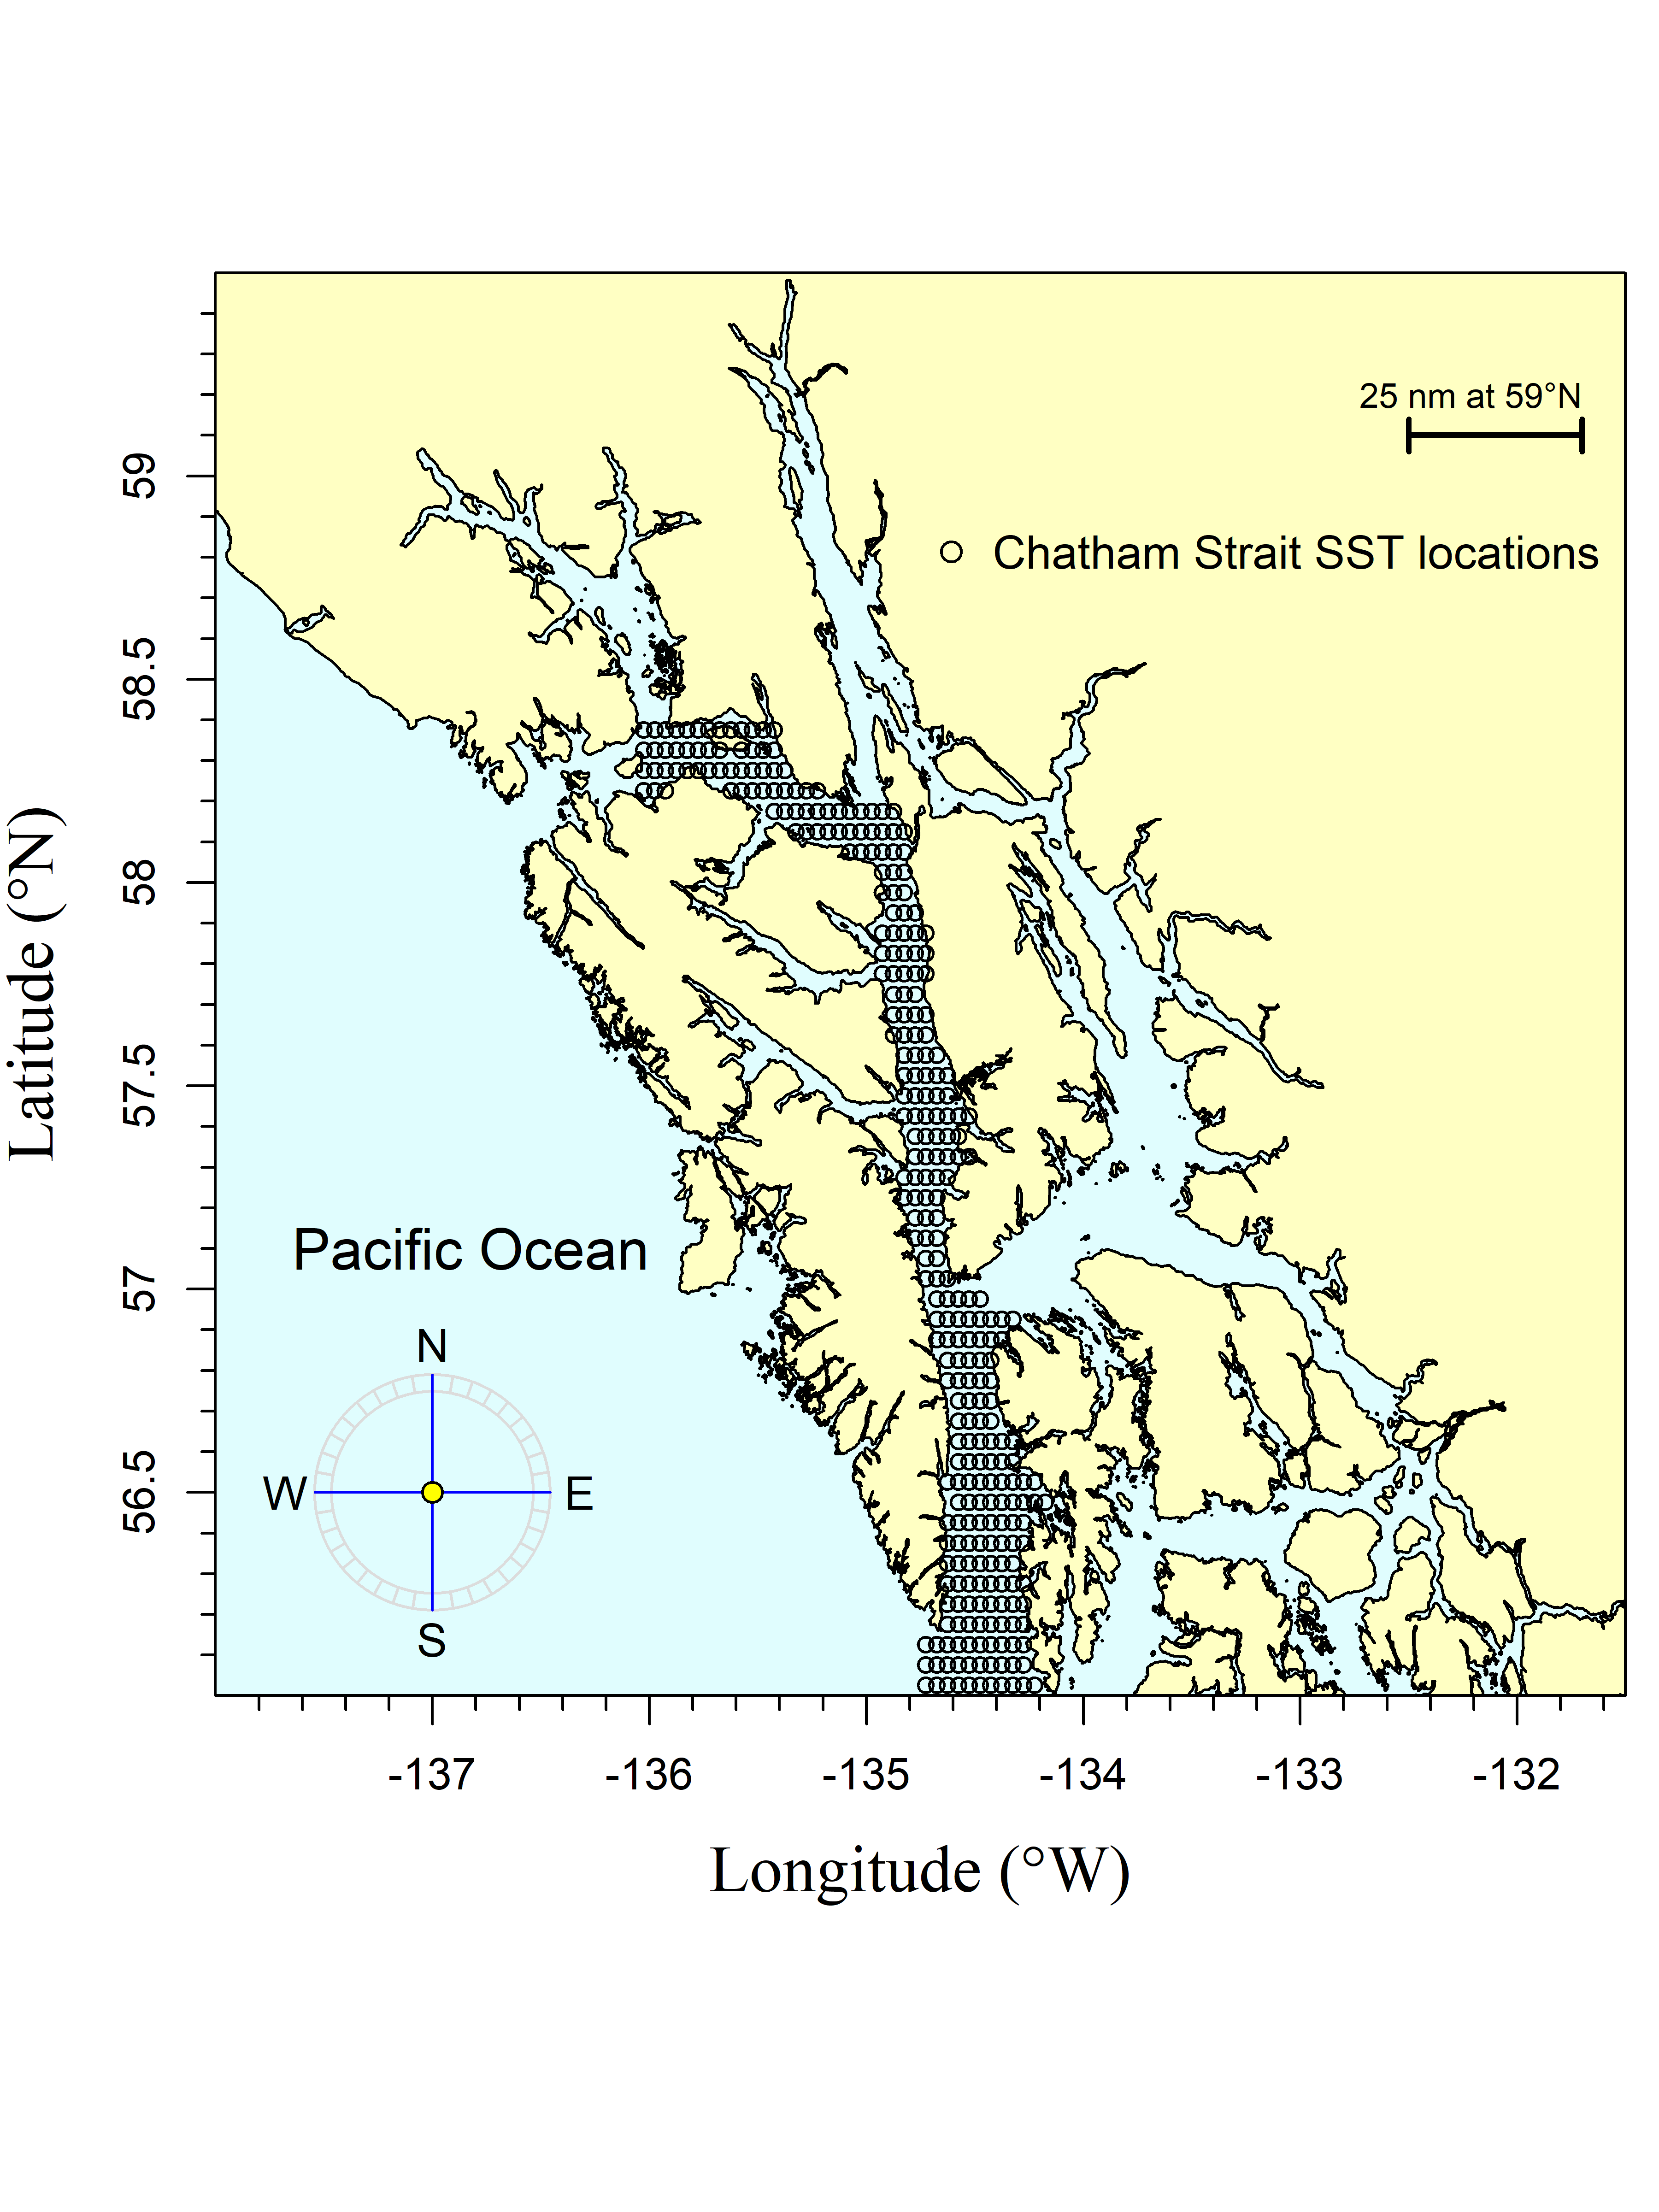
\includegraphics{../../2024_forecast/results/temperature_data/Chatham.png}
\caption{The Chatham and Icy Straits region encompasses waters of
Chatham and Icy Straits east of Lemesurier Island to Point Couverden,
south to the approximate latitude of 56.025 degrees north (roughly Cape
Decision off Kuiu Island). The black circles are the satellite stations
(i.e., data points).}
\end{figure}

\begin{figure}
\centering
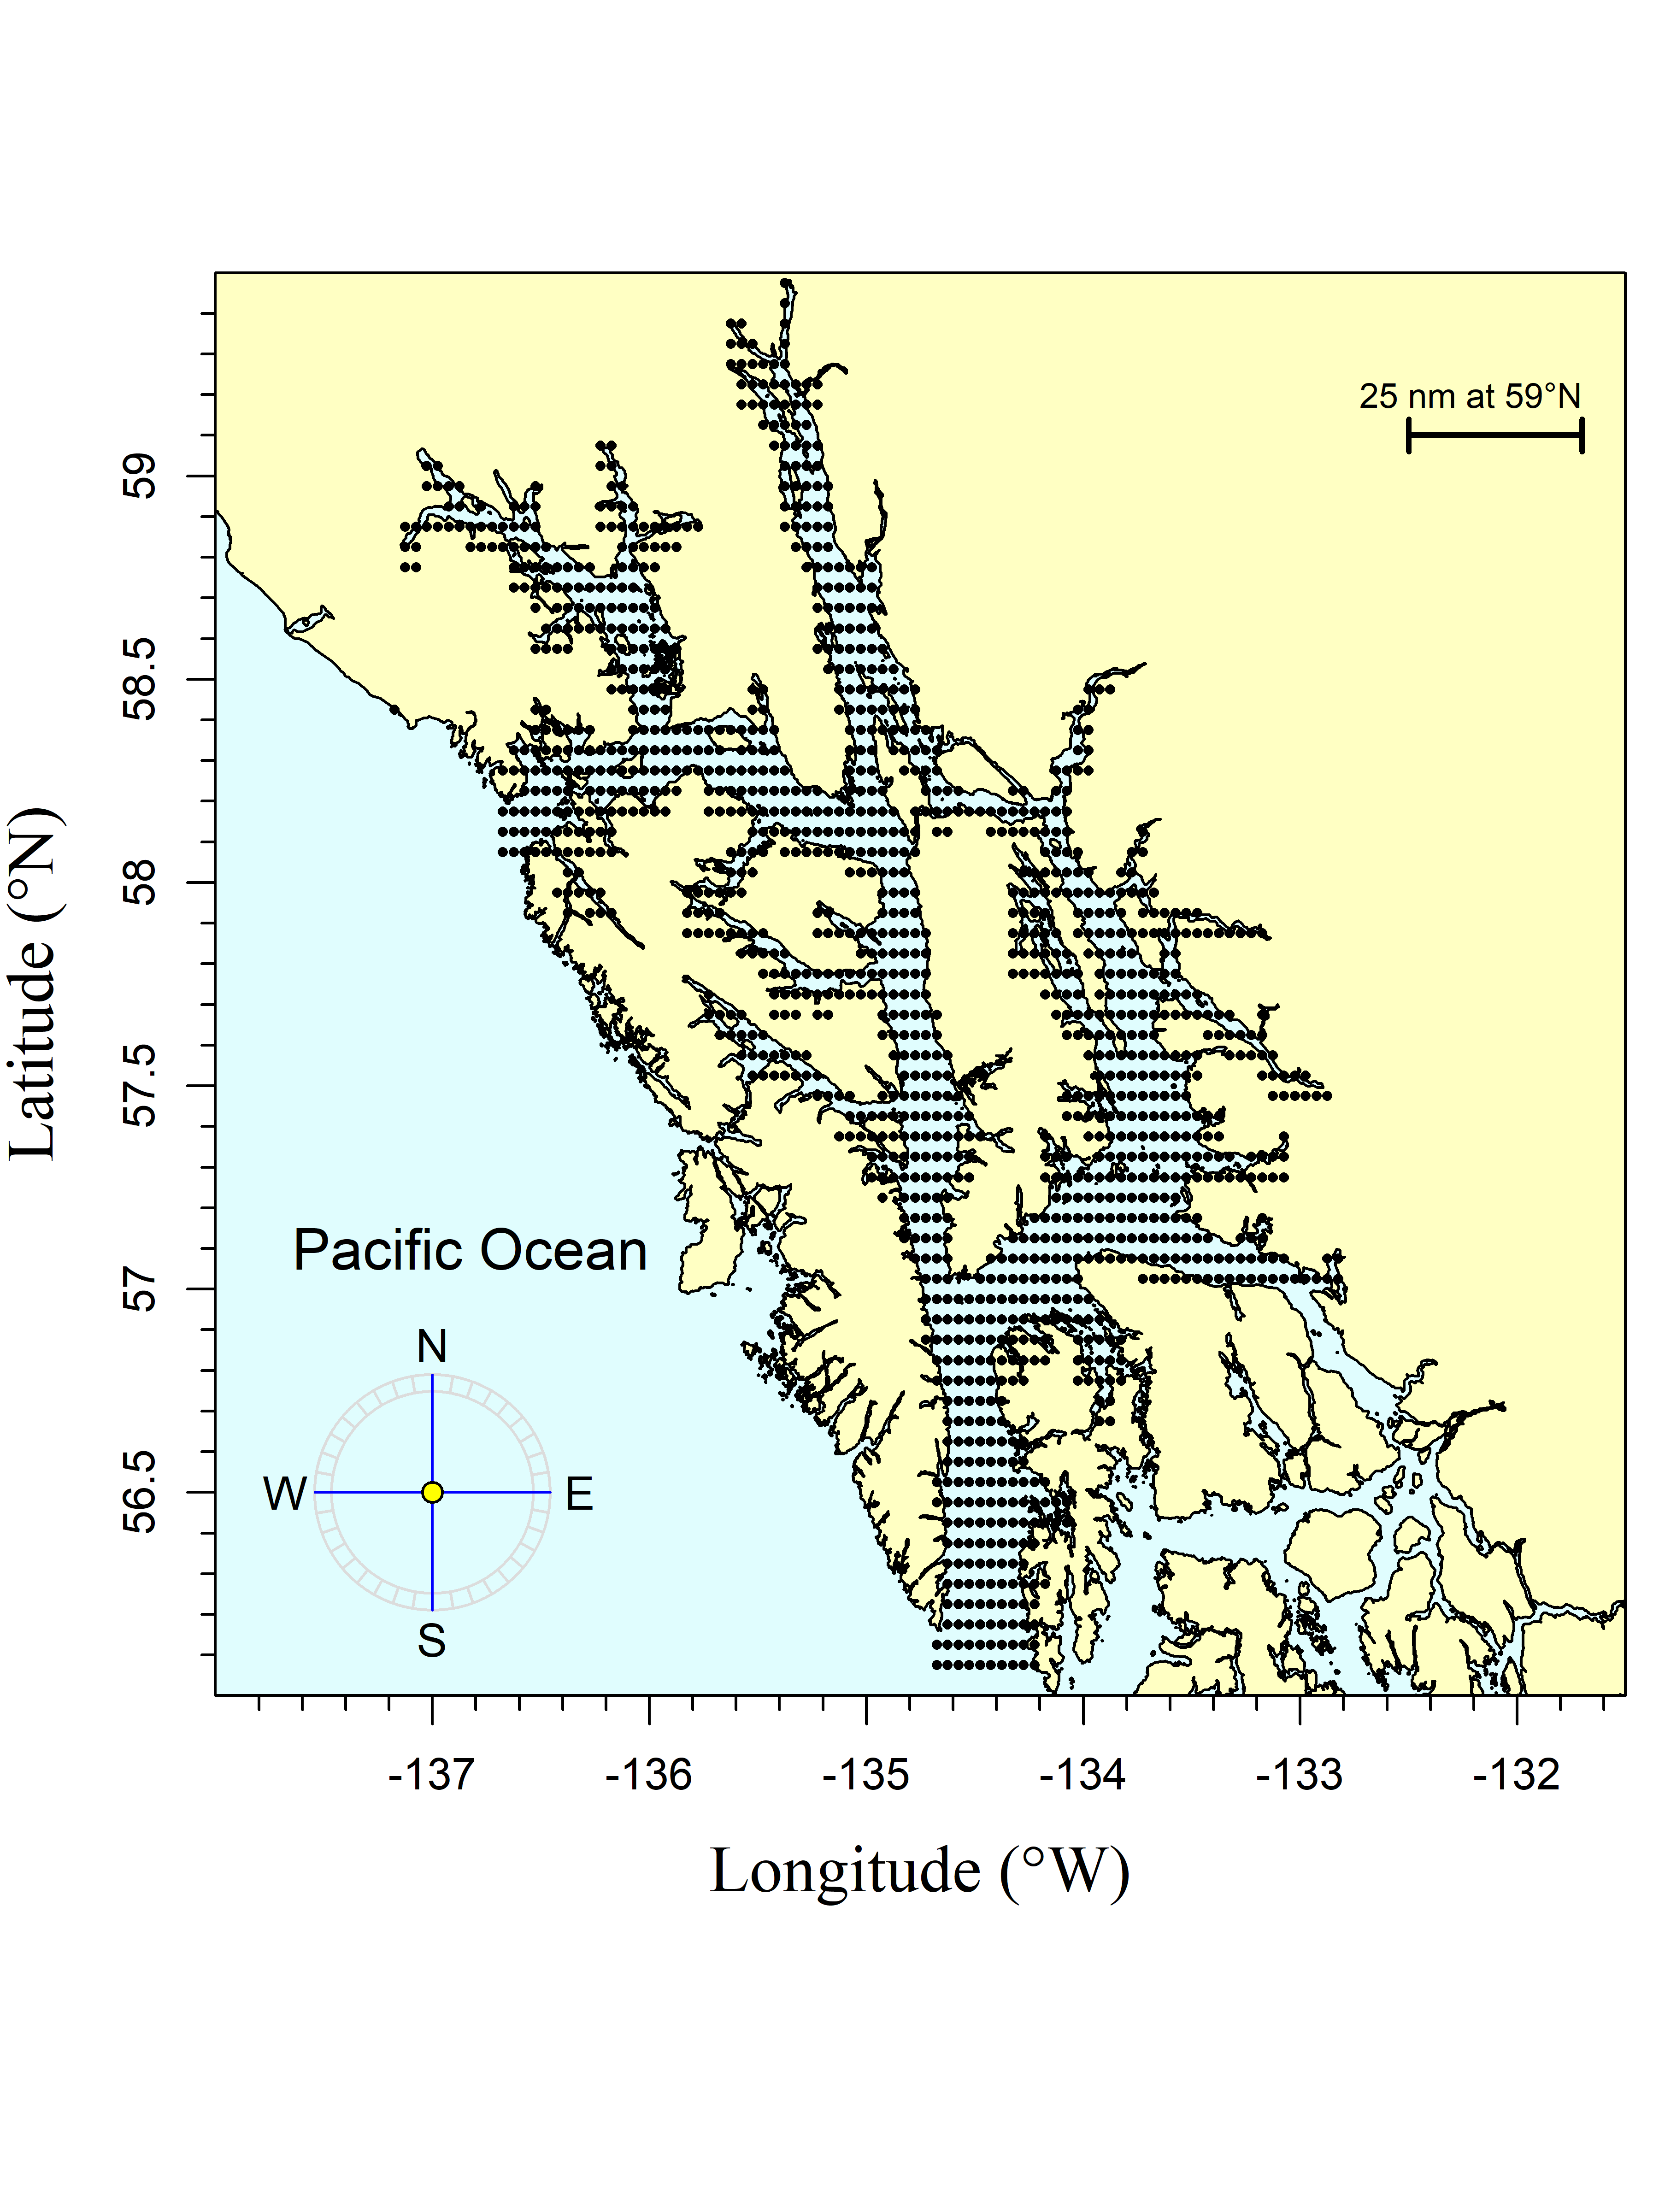
\includegraphics{../../2024_forecast/results/temperature_data/NSEAK.png}
\caption{The northern Southeast Alaska (NSEAK) region encompasses
northern Southeast Alaska from 59.475 to 56.075 degrees north latitude
and from -137.175 to -132.825 degrees west longitude. The black circles
are the satellite stations (i.e., data points).}
\end{figure}

\begin{figure}
\centering
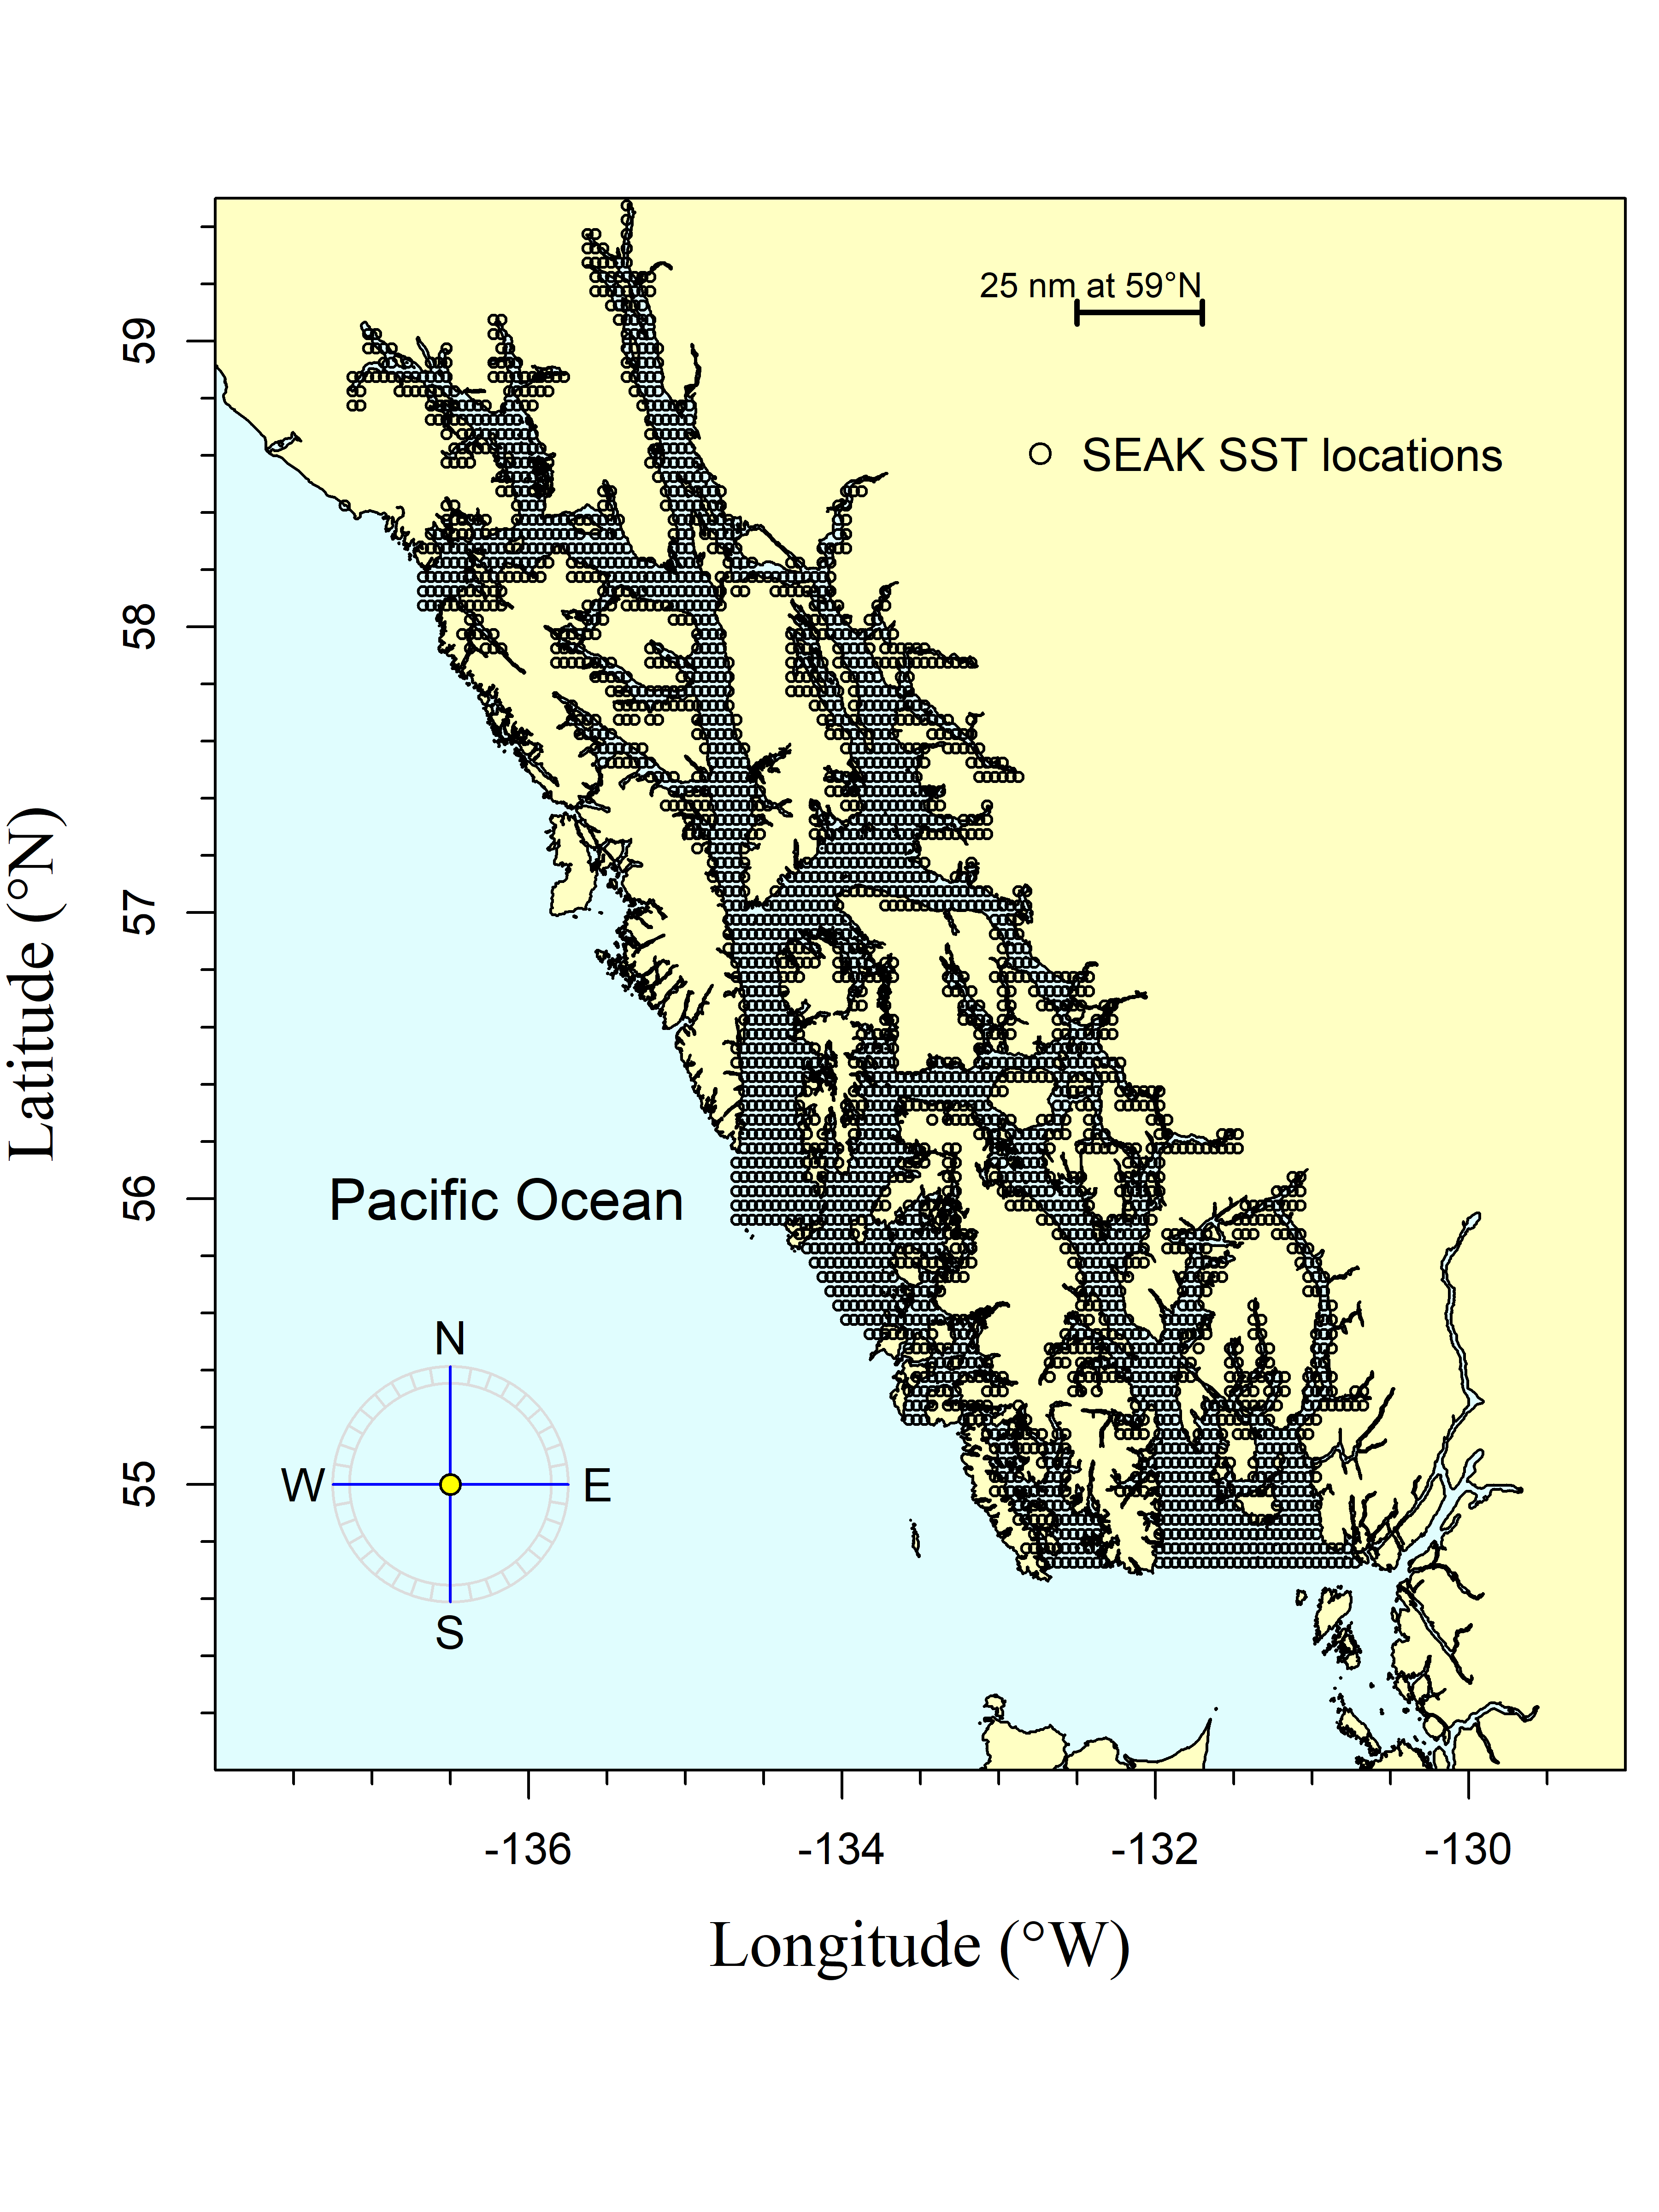
\includegraphics{../../2024_forecast/results/temperature_data/SEAK.png}
\caption{The Southeast Alaska (SEAK) region encompasses Southeast Alaska
from 59.475 to 54.725 degrees north latitude and from -137.175 to
-130.675 degrees west longitude. The black circles are the satellite
stations (i.e., data points).}
\end{figure}

\begin{figure}
\centering
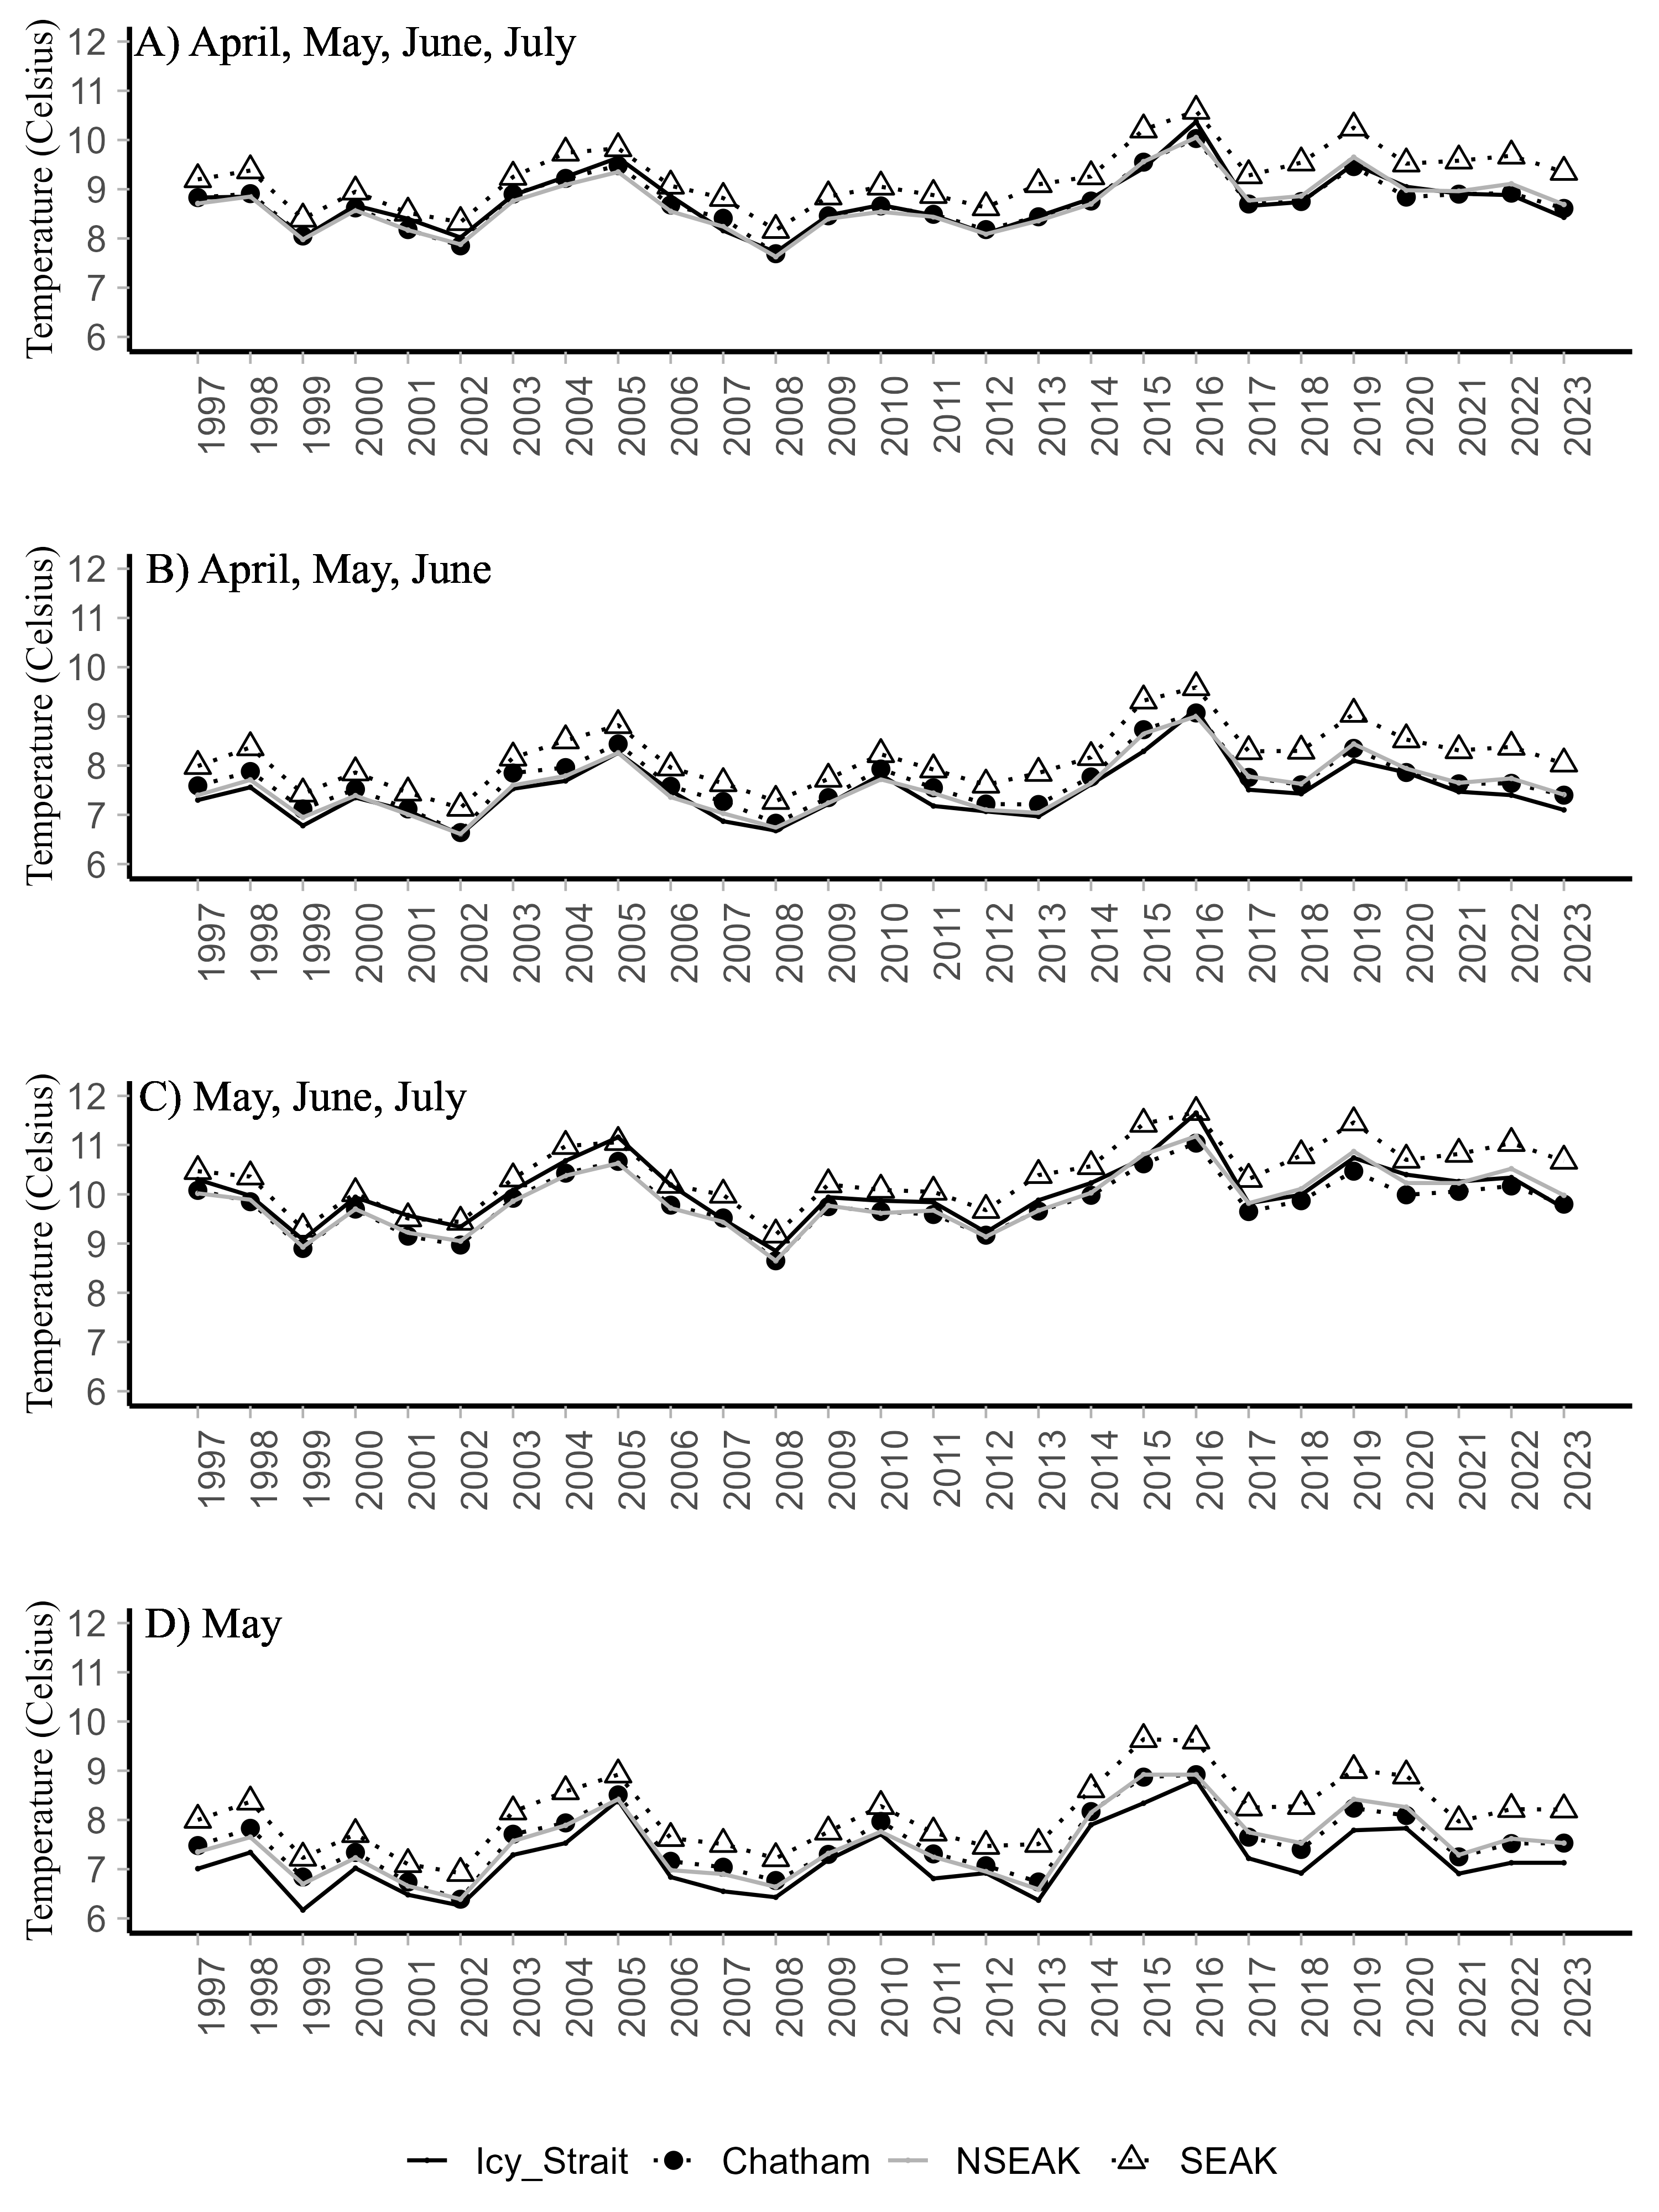
\includegraphics{../../2024_forecast/results/temperature_data/monthly_temp_regions.png}
\caption{A. The May temperature averaged over each region (Chatham and
Icy Straits, Icy Strait, NSEAK, SEAK) from 1997 through 2024. B. The
May, June, and July temperature averaged over each region (Chatham and
Icy Straits, Icy Strait, NSEAK, SEAK) from 1997 through 2024. C. The
April through June temperature averaged over each region (Chatham and
Icy Straits, Icy Strait, NSEAK, SEAK) from 1997 through 2024. D. The
April through July temperature averaged over each region (Chatham and
Icy Straits, Icy Strait, NSEAK, SEAK) from 1997 through 2024.}
\end{figure}

\begin{figure}
\centering
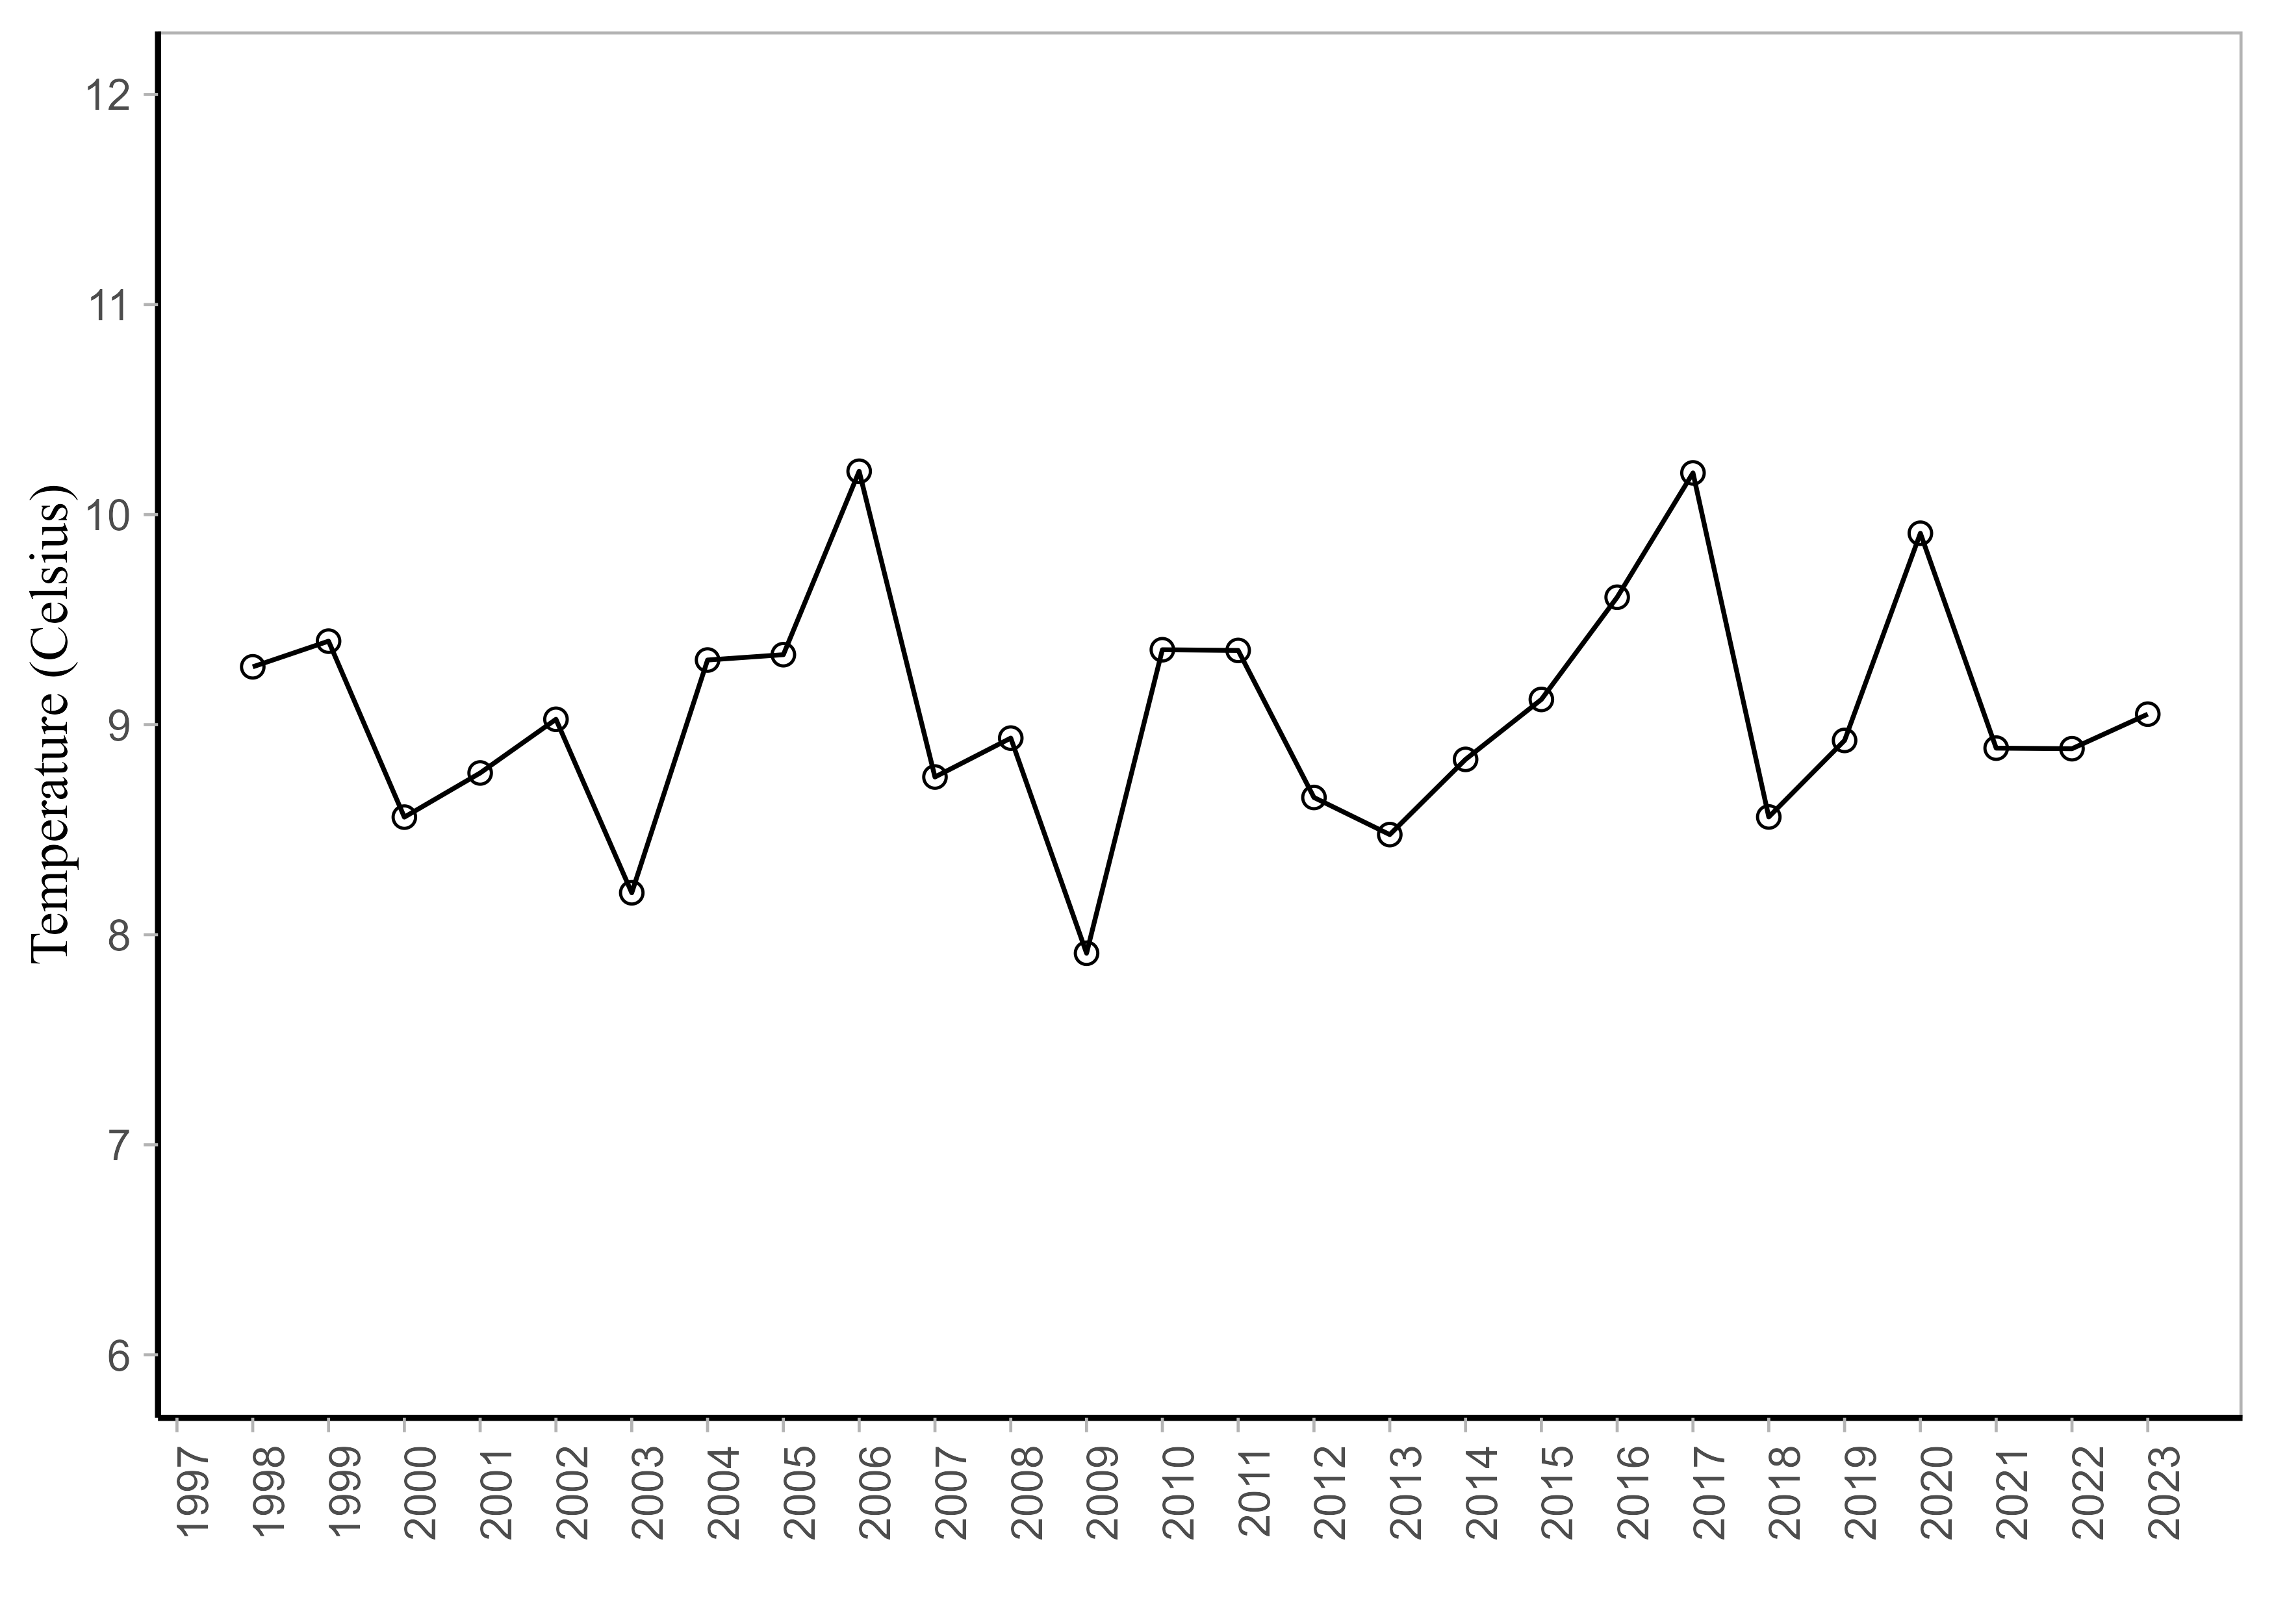
\includegraphics{../../2024_forecast/results/temperature_data/monthly_SECM_temp_regions.png}
\caption{Average temperature (degrees Celsius) at 20m during May, June,
and July at 8 stations in Icy Strait (Icy Strait and Upper Chatham
transects; ISTI) from 1997 through 2024.}
\end{figure}

\section{Acknowledgements}\label{acknowledgements}

Jordan Watson (NOAA) helped with the code to process the satellite data
into a usable format. The data was accessed through NOAA's Coral Reef
Watch
(\url{https://coastwatch.pfeg.noaa.gov/erddap/griddap/NOAA_DHW_monthly.html}
and
\url{https://coastwatch.pfeg.noaa.gov/erddap/griddap/NOAA_DHW.html}).
Emily Fergusson summarized the SECM survey data by year, month, and
depth. All code and associated data are located here:
\url{https://github.com/commfish/southeast_pink_salmon_preseason} in the
2024\_forecast folder.

\pagebreak

\section{References}\label{references}

Huang, B., P. W. Thorne, V. F. Banzon,, T. Boyer, G. Chepurin, J. H.
Lawrimore, M. J. Menne, T. M. Smith, R. S. Vose, and H. M. Zhang. 2017.
Extended reconstructed sea surface temperature, version 5 (ERSSTv5):
upgrades, validations, and intercomparisons. Journal of Climate
30:8179--8205.

NOAA Coral Reef Watch (NOAA\_DHW\_monthly dataset). 2022, updated daily.
NOAA Coral Reef Watch Version 3.1 Monthly 5km SST and SST Anomaly, NOAA
Global Coral Bleaching Monitoring Time Series Data, May 1997-June 2021.
College Park, Maryland, USA: NOAA/NESDIS/STAR Coral Reef Watch program.
Data set accessed 2022-09-12 at
\url{https://coastwatch.pfeg.noaa.gov/erddap/griddap/NOAA_DHW_monthly.html}.

NOAA Coral Reef Watch (NOAA\_DHW dataset). 2022, updated daily. NOAA
Coral Reef Watch Daily Near-real-Time Global 5km SST and SST Anomaly,
NOAA Global Coral Bleaching Monitoring Time Series Data, July 2021 to
July 2022. College Park, Maryland, USA: NOAA/NESDIS/STAR Coral Reef
Watch program. Data set accessed 2022-09-12 at
\url{https://coastwatch.pfeg.noaa.gov/erddap/griddap/NOAA_DHW.html}.

Piston, A. W., J. Murphy, J. Moss, W. Strasburger, S. C. Heinl, E.
Fergusson, S. Miller, A. Gray, and C. Waters. 2021. Operational Plan:
Southeast coastal monitoring, 2021. ADF\&G, Regional Operational Plan
No.~ROP.CF.1J.2021.02, Douglas.

\end{document}
